\section{Acceptance-Rejection Method}

The Acceptance-Rejection Method is a way to draw random deviates from a density function, $p(x)$. The steps are the following:
\begin{enumerate}
    \item Choose a function $f(x) > p(x)$ for all $x$ and make sure it is an integrable function.
    \item Calculate the total area of $f(x)$ and draw a uniform random deviate,$y \in [0,A_T]$.
    \item Evaluate the inverse function $f^{-1}(x)=F(y)$ to find $x_0$.
    \item Draw a second uniform random deviate, $f_1 \in[0,f(x_0)]$.
    \item Evaluate the density function $p(x_0)=p_1$ and if $f_1\leq p_1$, accept $x_0$ as a random deviate of the density function $p(x)$. Otherwise, reject the value and start process again.
\end{enumerate}

The set of accepted $x_0$ will map the density function $p(x)$. 

For this problem, we define p(x) to be the first half-cycle of a sine function (properly normalized) on the interval $[0,\pi]$ given by
\begin{equation}
    p(x)=\frac{1}{2}\sin{x},
    \label{eq:sinProb}
\end{equation}
For $f(x)$ we used two different functions: a constant and a quadratic function given by 
\begin{align}
    f(x)&=0.6\\
    f(x)&=-\frac{1}{5}x^2 + \frac{1}{5}x+0.05,
\end{align}
,respectively.

Then, they were integrated with respect to $x$ to find the following equations:
\begin{align}
    A(x)&=0.6x\\
    A(x)&=-\frac{1}{15}x^3 + \frac{1}{10}x^2 + 0.05x.
\end{align}
These equations were used determine the total area, $A_T$, for each function when evaluated at $x=\pi$. 

Additionally, they were used to determine a set of support points, $(A(x_i),x_i)$ which were used to do an interpolation and find an equivalent inverse function, $F(y)$. Note that for the interpolation the x's values are used as our y's and vice versa. 

After setting all of these functions we code the method inside a loop and run it N times. 

Figure \ref{fig:accRejPlot} compares the density function in orange, the chosen function for the method in green and the normalized histogram of the random deviates obtained with this method in blue. 
The red dots show the set of accepted pairs $(x_0,f_1)$. 
Using this figure we can visually attest that we have selected a function that is bigger than our density function for all $x$ in the interval.

Additionally, we can note that the number of iterations, N, affects the overall shape of the normalized histogram. 
At lower N, the full map of the distribution is not fully sampled so the histogram appears to not follow our desired distribution p(x). 
Nonetheless, we can verify that at larger N, we can completely map the density function space so the histogram correctly resembles our desired density function. 

The inefficiency factor was calculated by dividing the number of trials, N, over the number of accepted deviates. Table \ref{tab:accRej} shows that the inefficiency factor is almost equal to the total Area, $A_T$ and that the \\ quadratic function has an inefficiency factor smaller than the constant.

\begin{table}
    \centering
    \begin{subtable}{0.45\textwidth}
    \begin{tabular}{lrr}
\toprule
{} &  $Ineficiency Factor$ &  $TotalArea$ \\
\midrule
Constant  &                1.8727 &       1.8850 \\
Quadratic &                1.2107 &       1.1906 \\
\bottomrule
\end{tabular}

    \caption{N=1000}
    \end{subtable}
    \begin{subtable}{0.45\textwidth}
    \begin{tabular}{lrr}
\toprule
{} &  $Ineficiency Factor$ &  $TotalArea$ \\
\midrule
Constant  &                1.9080 &       1.8850 \\
Quadratic &                1.1898 &       1.1906 \\
\bottomrule
\end{tabular}

    \caption{N=10000}
    \end{subtable}
    \begin{subtable}{0.45\textwidth}
    \begin{tabular}{lrr}
\toprule
{} &  $Ineficiency Factor$ &  $TotalArea$ \\
\midrule
Constant  &                1.8869 &       1.8850 \\
Quadratic &                1.1935 &       1.1906 \\
\bottomrule
\end{tabular}

    \caption{N=50000}
    \end{subtable}
    \caption{Table that shows the total area and the inefficiency factor at different N values.}
    \label{tab:accRej}
\end{table}


\begin{figure*}
  \centering
  \begin{subfigure}[b]{0.3\textwidth}
    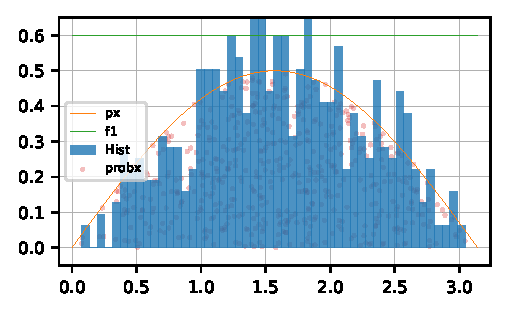
\includegraphics[scale=.66]{CodeAndFigures/AcceptanceRejectionPlotf1N1000.pdf}
    \caption{$f(x)=0.6, N=1000$}
    \label{subfig:consN1000}
  \end{subfigure}
    \begin{subfigure}[b]{0.3\textwidth}
    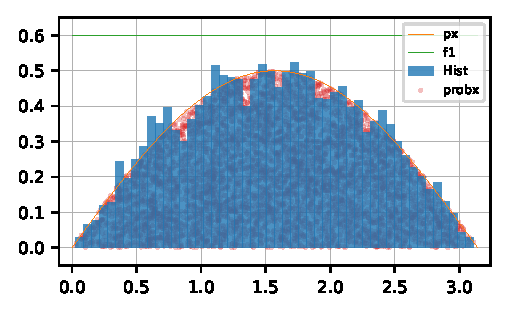
\includegraphics[scale=.66]{CodeAndFigures/AcceptanceRejectionPlotf1N10000.pdf}
    \caption{$f(x)=0.6, N=10000$}
    \label{subfig:consN10000}
  \end{subfigure}
    \begin{subfigure}[b]{0.3\textwidth}
    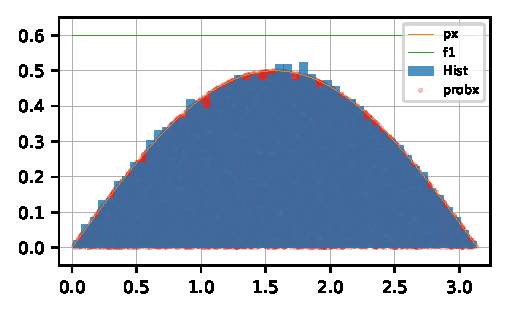
\includegraphics[scale=.66]{CodeAndFigures/AcceptanceRejectionPlotf1N50000.pdf}
    \caption{$f(x)=0.6, N=50000$}
    \label{subfig:consN50000}
  \end{subfigure}
  \begin{subfigure}[b]{0.3\textwidth}
    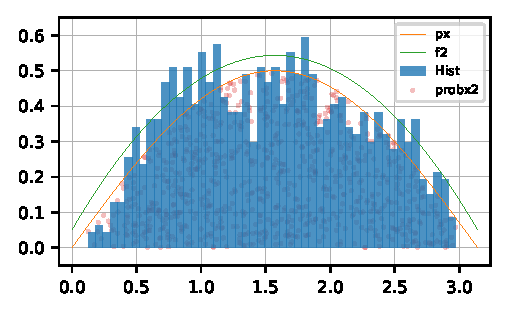
\includegraphics[scale=.66]{CodeAndFigures/AcceptanceRejectionPlotf2N1000.pdf}
    \caption{$f(x)=-.2x^2+.2x+.01$.}
    \label{subfig:QuadN1000}
  \end{subfigure}
    \begin{subfigure}[b]{0.3\textwidth}
    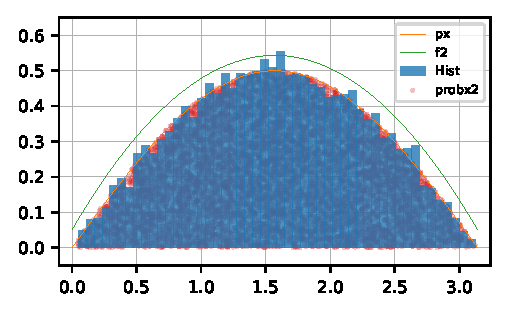
\includegraphics[scale=.66]{CodeAndFigures/AcceptanceRejectionPlotf2N10000.pdf}
    \caption{$f(x)=-.2x^2+.2x+.01$.}
    \label{subfig:QuadN10000}
  \end{subfigure}
    \begin{subfigure}[b]{0.3\textwidth}
    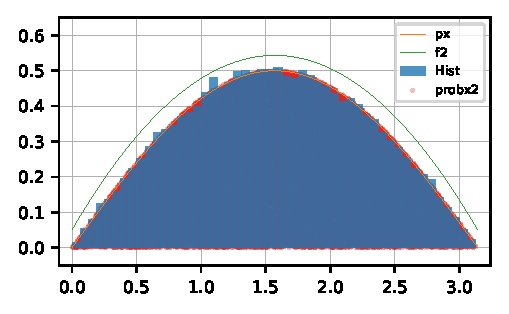
\includegraphics[scale=.66]{CodeAndFigures/AcceptanceRejectionPlotf2N50000.pdf}
    \caption{$f(x)=-.2x^2+.2x+.01$.}
    \label{subfig:QuadN50000}
  \end{subfigure}
  \caption{Plot of random deviates from a normalized sine function using the Acceptance/Rejection Method with [TOP ROW] constant function and [BOTTOM ROW] quadratic function. [FIRST COLUMN] N=1000, [2nd COLUMN] N=10000, [3rd COLUMN] N=50000.}
  \label{fig:accRejPlot}
\end{figure*}

% Use the Acceptance-Rejection Method to
% draw random deviates from a probability distribution shaped like the first half-cycle of a sine
% function (properly normalized) on the interval $[0,\pi]$.I would like you to use two different
% functions for $f(x)$:
% \begin{enumerate}
%     \item a constant $f(x)$ for the full interval
%     \item any other non-constant function of your choice.
% \end{enumerate}

% In each case you should compare the sine wave to a histogram your random deviates to show
% that you have faithfully sampled from the distribution. Finally, for each case show that the
% inefficiency factor (the number of trials you have to make divided by the number of good deviates
% that you get) is equal to the area under $f(x)$ on the interval $[0,\pi]$. Note that the function that
% you choose must have an efficiency factor that is smaller than that of the constant function.
